\documentclass[a4paper, 12pt]{article}

\usepackage{/Users/zhengz/Desktop/Math/Workspace/Homework1/homework}
%%%%%%%%%%%%%%%%%%%%%%%%%%%%%%%%%%%%%%%%%%%%%%%%%%%%%%%%%%%%%%%%%%%%%%%%%%%%%%%%%%%%%%%%%%%%%%%%%%%%%%%%%%%%%%%%%%%%%%%%%%%%%%%%%%%%%%%%
\begin{document}
%Header-Make sure you update this information!!!!
\noindent
%%%%%%%%%%%%%%%%%%%%%%%%%%%%%%%%%%%%%%%%%%%%%%%%%%%%%%%%%%%%%%%%%%%%%%%%%%%%%%%%%%%%%%%%%%%%%%%%%%%%%%%%%%%%%%%%%%%%%%%%%%%%%%%%%%%%%%%%
\large\textbf{Zhengdong Zhang} \hfill \textbf{Homework 2}   \\
Email: zhengz@uoregon.edu \hfill ID: 952091294 \\
\normalsize Course: MATH 635 - Algebraic Topology II \hfill Term: Winter 2025\\
Instructor: Dr.Daniel Dugger \hfill Due Date: $25^{th}$ January, 2025 \\
\noindent\rule{7in}{2.8pt}
\setstretch{1.1}

\begin{problem}{1}
Consider a map \(\alpha:(I^2,\partial I^2)\rightarrow (X,x)\) and the corresponding element \([\alpha]\) of \(\pi_2(X,x)\). The following picture depicts a map 
\(\beta:(I^2,\partial I^2)\rightarrow (X,x)\) which is "\(\alpha\) scaled down to a center cube of side-length \(\frac{1}{2}\), and the basepoint outside of that" (so the shaded region is all mapped to \(x\)):
\[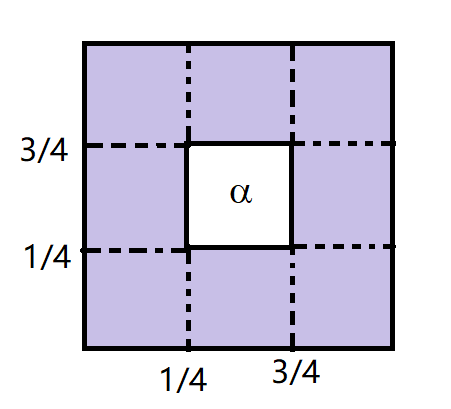
\includegraphics[scale=0.4]{Pictures/HW2-1.png}\]
\begin{enumerate}[(a)]
\item Write down an explicit formula for a map \(\lambda:I^2\rightarrow I^2\) such that \(\beta=\alpha\circ \lambda\).
\item Use the Convexity Lemma to give a rigorous proof (no handwaiving!) that \([\alpha]=[\beta]\) as elements of \(\pi_2(X,x)\).
\end{enumerate}
\end{problem}
\begin{solution}
\begin{enumerate}[(a)]
\item Write \(I^2=[0,1]\times [0,1]\). 
We first divide the purple part of the square in the problem into four regions:
\[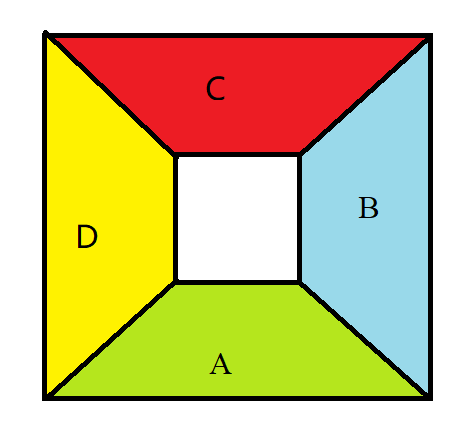
\includegraphics[scale=0.5]{Pictures/HW2-1-1.png}\]
\begin{itemize}
\item We say a point \((x,y)\) is in the region \(A\subset I^2\) if it satisfies one of the follwoing conditions: 
\begin{enumerate}[(1)]
\item \(0\leq y\leq x\leq \frac{1}{4}\);
\item \(\frac{1}{4}\leq x\leq \frac{3}{4}, 0\leq y\leq \frac{1}{4}\);
\item \(0\leq y\leq -x+1\leq \frac{1}{4}\).
\end{enumerate}  
\item We say a point \((x,y)\) is in the region \(B\subset I^2\) if it satisfies one of the following conditions:
\begin{enumerate}[(1)]
\item \(0\leq -x+1\leq y\leq \frac{1}{4}\);
\item \(\frac{1}{4}\leq x\leq 1, \frac{1}{4}\leq y\leq \frac{3}{4}\);
\item \(0\leq y-\frac{3}{4}\leq x-\frac{3}{4}\leq \frac{1}{4}\).
\end{enumerate}
\item We say a point \((x,y)\) is in the region \(C\subset I^2\) if it satisfies one of the following conditions:
\begin{enumerate}[(1)]
\item \(0\leq x-\frac{3}{4}\leq y-\frac{3}{4}\leq \frac{1}{4}\);
\item \(\frac{1}{4}\leq x\leq \frac{3}{4}, \frac{3}{4}\leq y\leq 1\);
\item \(0\leq 1-y\leq x\leq \frac{1}{4}\).
\end{enumerate}
\item We say a point \((x,y)\) is in the region \(D\subset I^2\) if it satisfies one of the following conditions:
\begin{enumerate}[(1)]
\item \(0\leq x\leq 1-y\leq \frac{1}{4}\);
\item \(0\leq x\leq \frac{1}{4},\frac{1}{4}\leq y\leq \frac{3}{4}\);
\item \(0\leq x\leq y\leq \frac{1}{4}\).
\end{enumerate}
\end{itemize}
We define a continous map \(\lambda:I^2\rightarrow I^2\) as follows
\[\lambda(x,y)=\begin{cases}
    (\frac{1}{2}-\frac{1}{2}\frac{2x-1}{2y-1},0),&\, \text{if}\, (x,y)\in A;\\[5pt]
    (1,\frac{1}{2}+\frac{1}{2}\frac{2y-1}{2x-1}),&\, \text{if}\, (x,y)\in B;\\[5pt]
    (\frac{1}{2}+\frac{1}{2}\frac{2x-1}{2y-1},1),&\, \text{if}\, (x,y)\in C;\\[5pt]
    (0,\frac{1}{2}-\frac{1}{2}\frac{2y-1}{2x-1}),&\, \text{if}\, (x,y)\in D;\\[5pt]
    (2x-\frac{1}{2},2y-\frac{1}{2}),&\, \text{if}\, \frac{1}{4}\leq x,y\leq \frac{3}{4}.
\end{cases}\]
This map \(\lambda\) sends the points in the purple square to the boundary and stretch the middle white square to the whole square, so we have \(\beta=\alpha\circ \lambda\).
\item \((I^2,\partial I^2)\) is a pair of spaces where \(I^2\) is a convex set in \(\mathbb{R}^2\) and \(id,\lambda:I^2\rightarrow I^2\) are both maps from \(I^2\) to \(I^2\).  When restricted to the boundary \(\partial I^2\), both 
\(id\) and \(\lambda\) is the identity \(\partial I^2\rightarrow \partial I^2\). By the Convexity Lemma, we have \(\lambda\simeq id\) rel. \(\partial I^2\). This implies that 
\[\beta=\alpha\circ \lambda \simeq\alpha\circ id=\alpha\,\,\, \text{rel.}\,\, \partial I^2.\]
Thus, \(\alpha\) and \(\beta\) are homotopic relative to \(\partial I^2\) and they represent the same element \([\alpha]=[\beta]\) in the homotopy group \(\pi_2(X,x)\).
\end{enumerate}
\end{solution}

\noindent\rule{7in}{2.8pt}

\begin{problem}{2}
Let \(f:(I,\partial I)\rightarrow (X,x)\) be a based loop, and let \(\bar{f}:I\rightarrow X\) be the loop \(\bar{f}(t)=f(1-t)\). Use the Convexity Lemma to give a rigorous and brief proof that 
\(\bar{f}*f\) is homotopic rel \(\partial I\) to the constant loop at \(x\).
\end{problem}
\begin{solution}
Write \(I=[0,1]\) and define a map \(\lambda:I\rightarrow I\) as follows:
\[\lambda(t)=\begin{cases}
    2t,&\, \text{if}\, 0\leq t\leq \frac{1}{2},\\ 
    -2t+2&\, \text{if}\, \frac{1}{2}\leq t\leq 1.
\end{cases}\]
\(\lambda\) is continous and we have
\[(\bar{f}*f)(t)=(f\circ \lambda)(t)=\begin{cases}
    f(2t),&\, \text{if}\, 0\leq t\leq \frac{1}{2},\\ 
    \bar{f}(2t-1)=f(-2t+2),&\, \text{if}\, \frac{1}{2}\leq t\leq 1.
\end{cases}\]
Consider the constant map \(C_0:I\rightarrow I\) which maps everything to \(0\in I\) and we have 
\[C_0(0)=0=\lambda(0)\,\,\, ,C_0(1)=0=\lambda(1).\]
By the Convexity Lemma, we have 
\[C_0\simeq \lambda\,\, \text{rel.}\,\, \partial I.\]
This implies that 
\[\bar{f}*f=f\circ \lambda\simeq f\circ C_0=C_x\,\, \text{rel}\,\, \partial I\]
where \(C_x:I\rightarrow X\) is the constant map which sends everything to \(x\in X\). 
\end{solution}

\noindent\rule{7in}{2.8pt}


\begin{problem}{3}
Find the flaw in the following "proof" that \(0=1\):
Fix a natural number \(n\), and let \(j:S^n\hookrightarrow \mathbb{R}^{n+1}-0\) be the inclusion. Of course \(j\) is a homotopy equivalence. If \(f,g:S^n\rightarrow S^n\) are any two maps notice that \(jf\simeq jg \) via the straight-line 
homotopy \(H:S^n\times I\rightarrow \mathbb{R}^{n+1}-0\) given by 
\[H(x,t)=(1-t)\cdot f(x)+t\cdot g(x)\]
since obviously \(H_0=jf\) and \(H_1=jg\). Now look at the two composites 
\begin{align*}
    H_n(S^n)&\xrightarrow{f_*}H_n(S^n)\xrightarrow{j_*}H_n(\mathbb{R}^{n+1}-0),\\ 
    H_n(S^n)&\xrightarrow{g_*}H_n(S^n)\xrightarrow{j_*}H_n(\mathbb{R}^{n+1}-0).
\end{align*}
We know \(j_*f_*=(jf)_*=(jg)_*=j_*g_*\) since \(jf\) is homotopic to \(jg\). But \(j_*\) is an isomorphism because \(j\) is a homotopy equivalence, therefore \(f_*=g_*\). So any two maps \(f,g:S^n\rightarrow S^n\) has the same degree. 
In particular, if we take \(f\) to be a constant map and \(g\) to be the identity, then we obtain \(0=1\). 
\end{problem}
\begin{solution}
The flaw is the following:\\ 
When we prove that \(jg\simeq jf\) using the straight-line homotopy, the image of this homotopy \(H\) may contain the point \(0\in \mathbb{R}^{n+1}\). This means \((jf)_*\) is not necessarily equal to \((jg)_*\) as both the space \(S^n\) and 
\(\mathbb{R}^{n+1}-0\) do not contain the point \(0\). The straight-line homotopy we use may not be a homotopy for \(jf,jg:S^n\rightarrow \mathbb{R}^{n+1}-0\).

In the case \(f\) is the constant map \(f(S^n)=p\) and \(g\) is the identity. Consider the antipodal point \(-p\) and the straight-line homotopy \(H(x,t)\), we have 
\[H(-p,1/2)=(1-1/2)p+(-p)\cdot 1/2=0.\]
So this homotopy is not well-defined.
\end{solution}

\noindent\rule{7in}{2.8pt}

\begin{problem}{4}
Let \(X\) and \(Y\) be two spaces, with basepoint \(x\in X\) and \(y\in Y\). Prove that when \(n\geq 1\) there is an isomorphism of groups 
\[\pi_n(X\times Y,(x,y))\cong \pi_n(X,x)\times \pi_n(Y,y).\]
\end{problem}
\begin{solution}
Consider the projection maps \(p_X:X\times Y\rightarrow X\) and \(p_Y:X\times Y\rightarrow Y\). We have \(p_X(x,y)=x\) and \(p_Y(x,y)=y\). This induces two maps 
\begin{align*}
    (p_X)_*:&\pi_n(X\times Y,(x,y))\rightarrow \pi_n(X,x),\\ 
    (p_Y)_*:&\pi_n(X\times Y,(x,y))\rightarrow \pi_n(Y,y).
\end{align*}
Define 
\[p=(p_X)_*\times (p_Y)_*:\pi_n(X\times Y,(x,y))\rightarrow \pi_n(X,x)\times \pi_n(Y,y).\]
This is a group homomorphism since both \((p_X)_*\) and \((p_Y)_*\) are group homomorphisms. We need to show that \(p\) is both injective and surjective. 
\begin{itemize}
\item Let \(\gamma:(I^n,\partial I^n)\rightarrow (X\times Y,(x,y))\) be a continous map and \([\gamma]\) is corresponding element in \(\pi_n(X\times Y,(x,y))\). Assume \([\gamma]\in \ker p\). This means 
\(p([\gamma])=([C_x],[C_y])\) where \(C_x:(I^n,\partial I^n)\rightarrow (X,x)\) and \(C_y:(I^n,\partial I^n)\rightarrow (Y,y)\) are the constant maps. By definition, we have the composition 
\(I^n\xrightarrow{\gamma} X\times Y\xrightarrow{p_X} X\) is homotopic to the constant map \(C_x\) and \(I^n\xrightarrow{\gamma}X\times Y\xrightarrow{p_Y} Y\) is homotopic to the constant map \(C_y\). Since \(p_X\) and \(p_Y\) are only 
projections, so \(\gamma:I^n\rightarrow X\times Y\) is homotopic to the constant map \(C_{x,y}\) sending everything in \(I^n\) to the point \((x,y)\) via the product of the previous two homotopies. This shows that \([\gamma]\) is the identity element in \(\pi_n(X\times Y,(x,y))\). So 
\(p\) is injective.
\item Suppose \(([\gamma_1],[\gamma_2])\in \pi_n(X,x)\times \pi_n(Y,y)\) is an element represented by \(\gamma_1:I^n\rightarrow X\) and \(\gamma_2:I^n\rightarrow Y\). Define a map 
\begin{align*}
    \gamma:I&\rightarrow X\times Y,\\ 
    t&\mapsto (\gamma_1(t),\gamma_2(t)).
\end{align*}
We know that the corresponding homotopy class \([\gamma]\) is an element in \(\pi_n(X\times Y,(x,y))\) and we have 
\[p([\gamma])=((p_X)_*[\gamma],(p_Y)_*[\gamma])=([p_X\circ \gamma],[p_Y\circ \gamma])=([\gamma_1],[\gamma_2]).\]
This proves that \(p\) is surjective.
\end{itemize}
\end{solution}

\noindent\rule{7in}{2.8pt}
\newpage
\begin{problem}{5}
\begin{enumerate}[(a)]
\item Let \(T\) be the torus and \(M\) be the M\"{o}bius band. Let \(X\) be the space obtained by gluing the boundary of \(M\) homeomorphically to the "diagonal" circle on the torus (when viewing the torus as a quotient 
space of \(I^2\) in the standard way, this is the usual diagonal). Compute \(H_*(X)\).
\item Start with the usual model of \(\mathbb{R}P^2\) where we have a disk \(D^2\) with antipodal points on the boundary identified. Drill a triangular hole in the middle of the disk and label the side \(\beta\), \(\beta\), and \(\beta\) (all oriented 
clockwise), and let \(Y\) be the resulting quotient space: 
\[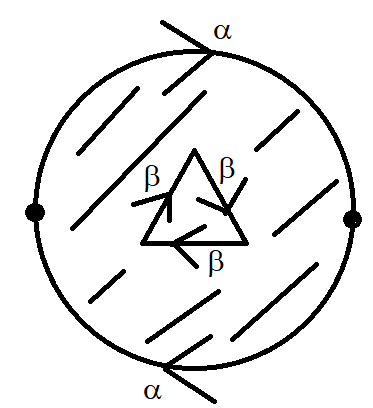
\includegraphics[scale=0.5]{Pictures/HW2-2.png}\]
Determine \(H_*(Y)\).
\newpage 
\item Repeat part (b) where the hole is a square rather than a triangle, and where the four sides are again all labelled with \(\beta\) and all oriented clockwise.
\[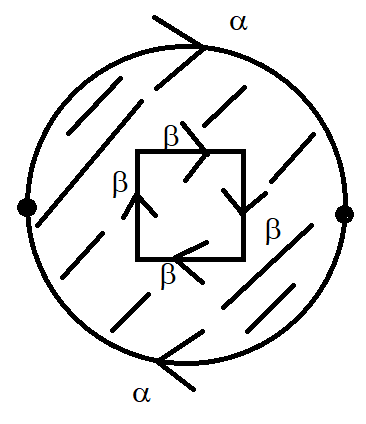
\includegraphics[scale=0.5]{Pictures/HW2-3.png}\]
\end{enumerate}
\end{problem}
\begin{solution}
\begin{enumerate}[(a)]
\item We use the following cell complex structure:
\[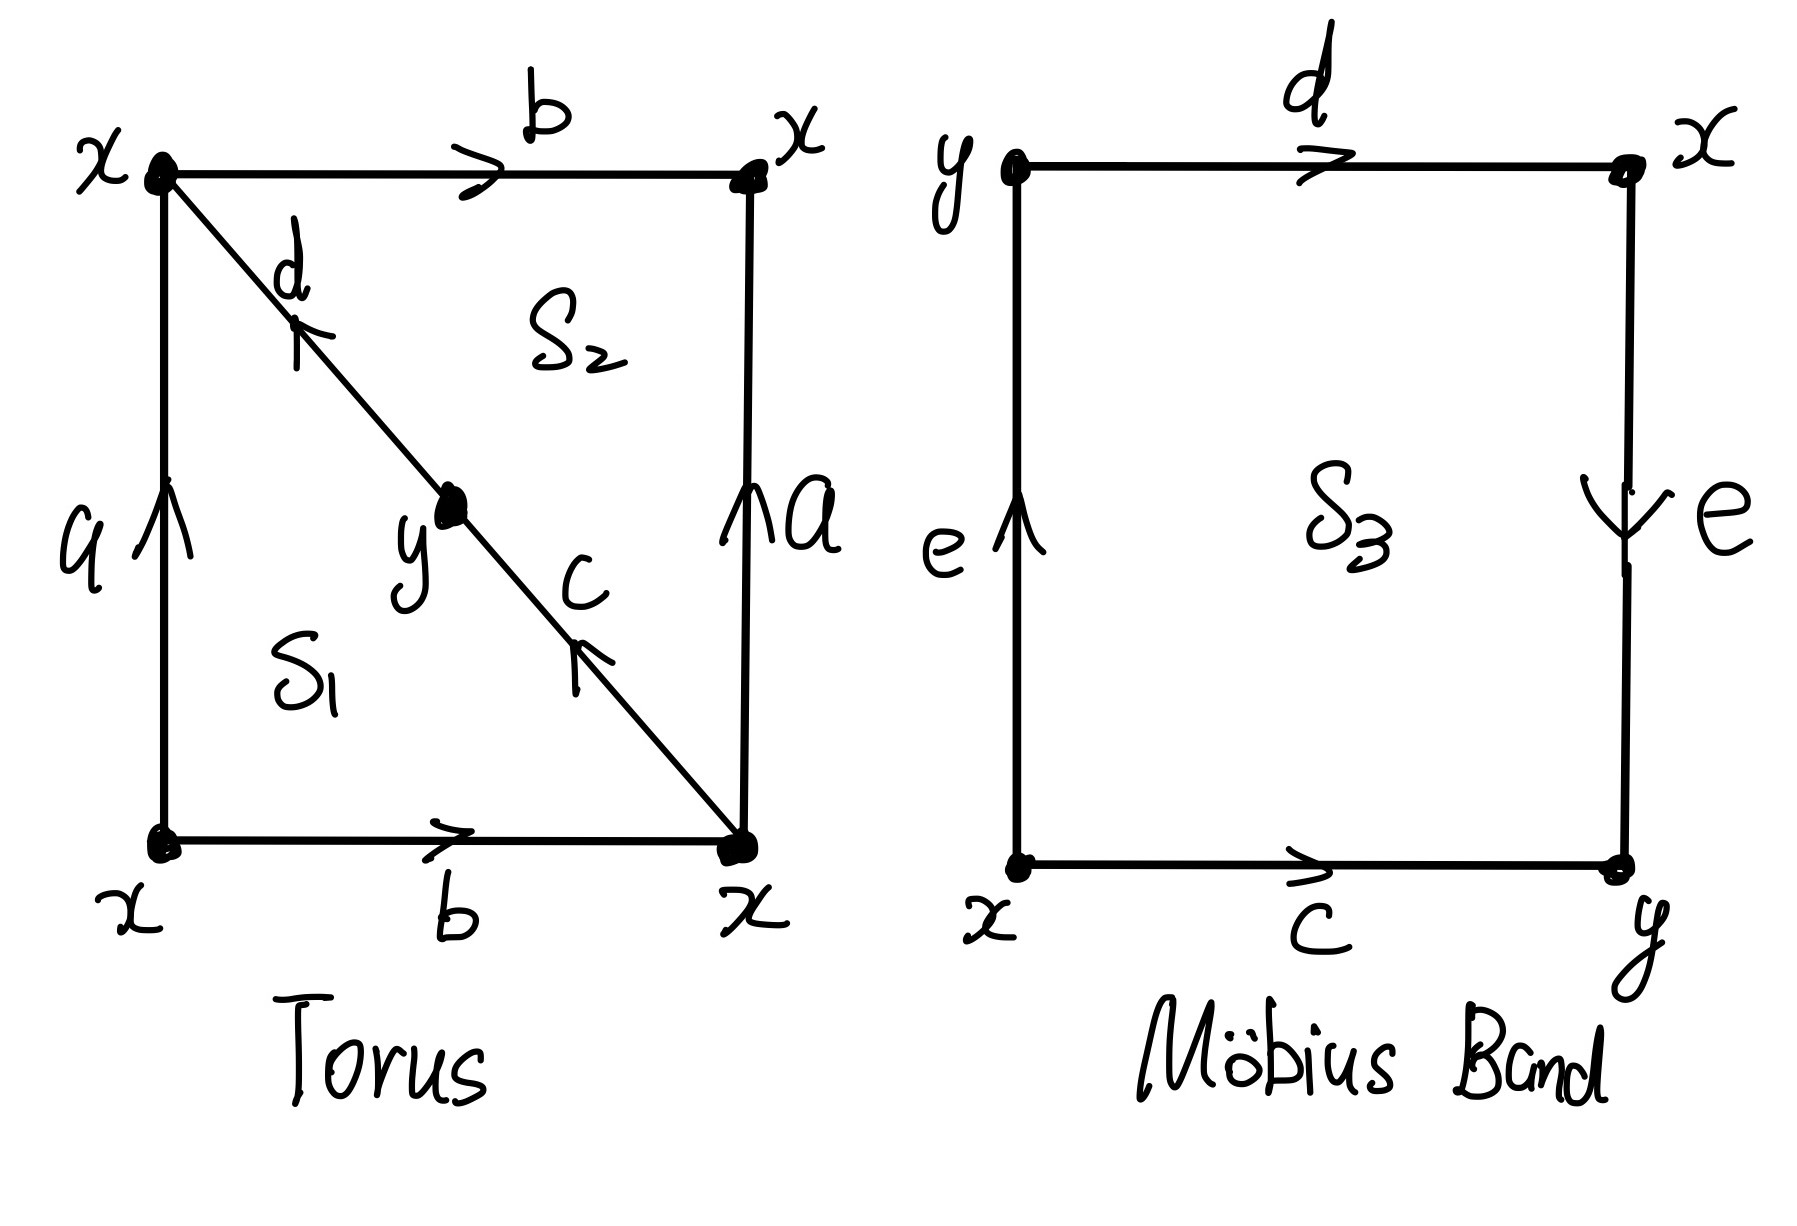
\includegraphics[scale=0.1]{Pictures/HW2-4.jpg}\]
The space \(X\) has two 0-cells \(x,y\), five 1-cells \(a,b,c,d,e\) and three 2-cells \(S_1,S_2,S_3\). We have the following cellular chain complex:\
\[\mathbb{Z}^3\xrightarrow{d_2}\mathbb{Z}^5\xrightarrow{d_1}\mathbb{Z}^2\xrightarrow{d_0}0\]
where \(d_0(x)=d_0(y)=0\) and 
\begin{align*}
    &d_1(a)=d_1(b)=x-x=0,\,\, &d_2(S_1)=-a+b+c+d,\\ 
    &d_1(c)=d_1(e)=y-x,\,\, &d_2(S_2)=c+d+b-a,\\ 
    &d_1(d)=x-y,\,\, &d_2(S_3)=2e+d-c.
\end{align*}
We can see that 
\begin{align*}
\ker d_1&=\la a,b,c+d,e+d\ra,\\ 
\im  d_1&=\la x-y\ra,\\
\ker d_2&=\la S_1-S_2\ra,\\ 
\im  d_2&=\la a-b-c-d,2e+d-c.\\ 
\ker d_0&=\la x,y\ra.
\end{align*}
We can calculate the homology group:
\begin{align*}
H_0(X)&=\ker d_0/\im d_1 \\
      &=\la x,y\ra/\la x-y\ra\\ 
      &=\mathbb{Z},\\ 
H_2(X)&=\ker d_2\\ 
      &=\la S_1-S_2\ra \\ 
      &=\mathbb{Z}.
\end{align*}
and 
\begin{align*}
    H_1(X)&=\ker d_1/\im d_2 \\ 
      &=\la a,b,c+d,e+d\ra/\la a-b-c-d,2e+d-c\ra\\ 
      &= \la b,a-b,e-c,c+d\ra/\la a-b-c-d,2e+d-c\ra\\
      &=\la b,c+d,e-c,a-b-c-d\ra/\la a-b-c-d,2(e-c)+c+d\ra\\ 
      &=\la b, u, v\ra/\la u+2v\ra\\ 
      &=\la b,u+v,v\ra/\la (u+v)+v\ra\\ 
      &=\mathbb{Z}\oplus \mathbb{Z}
\end{align*}
So the homology group of \(X\) can be summarized as 
\[H_i(X)=\begin{cases}
    \mathbb{Z},&\, \text{if}\, i=0,2;\\ 
    \mathbb{Z}\oplus \mathbb{Z},&\, \text{if}\, i=1;\\ 
    0,&\, \text{otherwise}.
\end{cases}\]
\item consider the following cell complex structure:
\[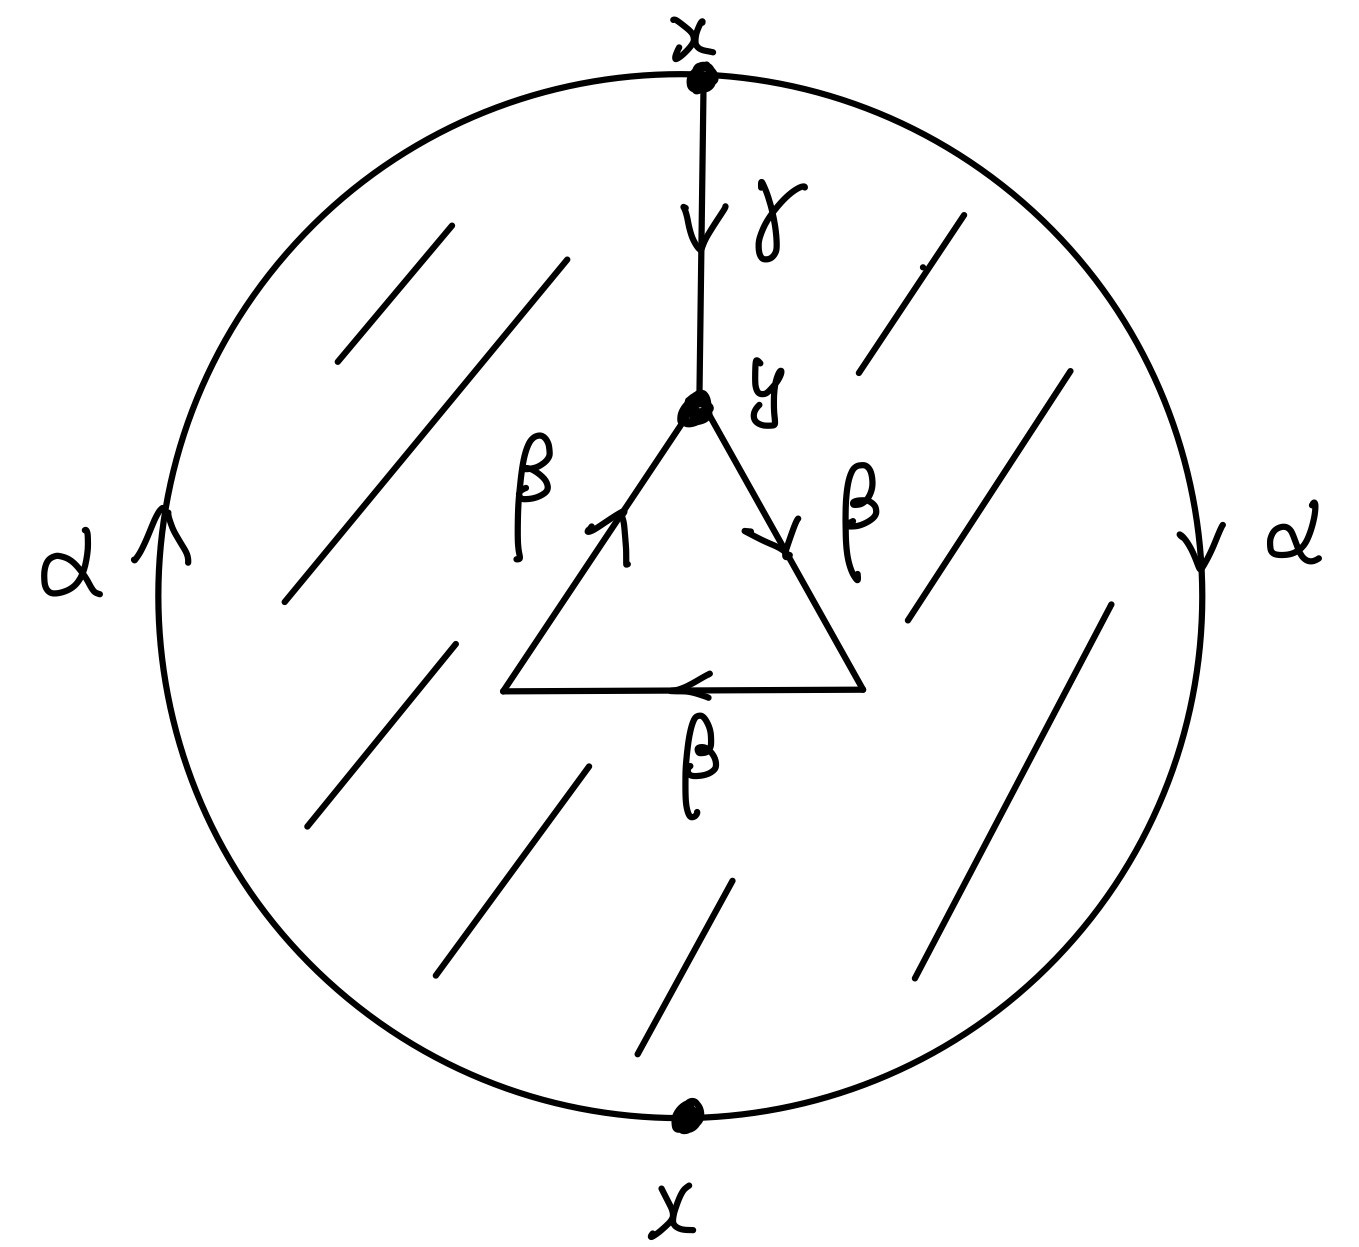
\includegraphics[scale=0.1]{Pictures/HW2-2-1.jpg}\]
The space \(Y\) has two 0-cells \(x,y\), three 1-cells \(\alpha,\beta,\gamma\) and one 2-cell \(S\). We have the following cellular complex:
\[\mathbb{Z}\xrightarrow{d_2}\mathbb{Z}^3\xrightarrow{d_1}\mathbb{Z}^2\xrightarrow{d_0}0.\]
The boundary maps are given by 
\begin{align*}
    d_2(S)&=2\alpha+\gamma-3\beta-\gamma=2\alpha-3\beta,\\ 
    d_1(\alpha)&=d_1(\beta)=0,\\ 
     d_1(\gamma)&=y-x,\\ 
    d_0&=0
\end{align*}
So we can calculate the homology groups 
\[H_2(Y)=\ker d_2=0.\]
\begin{align*}
    H_0(Y)&=\ker d_0/\im d_1\\ 
          &=\la x,y\ra/\la y-x\ra\\ 
          &=\mathbb{Z}
\end{align*}
and 
\begin{align*}
H_1(Y)&=\ker d_1\im d_2\\ 
      &=\la \alpha,\beta\ra/\la 2\alpha-3\beta\ra\\ 
      &=\la \alpha-\beta,\beta\ra/\la 2(\alpha-\beta)-\beta\ra\\ 
      &=\la \alpha-\beta,\alpha-2\beta\ra/\la \alpha-\beta+\alpha-2\beta\ra\\ 
      &=\mathbb{Z}.
\end{align*}
So the homology group of \(Y\) can be summarized as 
\[H_i(Y)=\begin{cases}
    \mathbb{Z},&\, \text{if}\, i=0,1;\\ 
    0,&\, \text{otherwise}.
\end{cases}\]
\item Now the cell structure is like this:
\[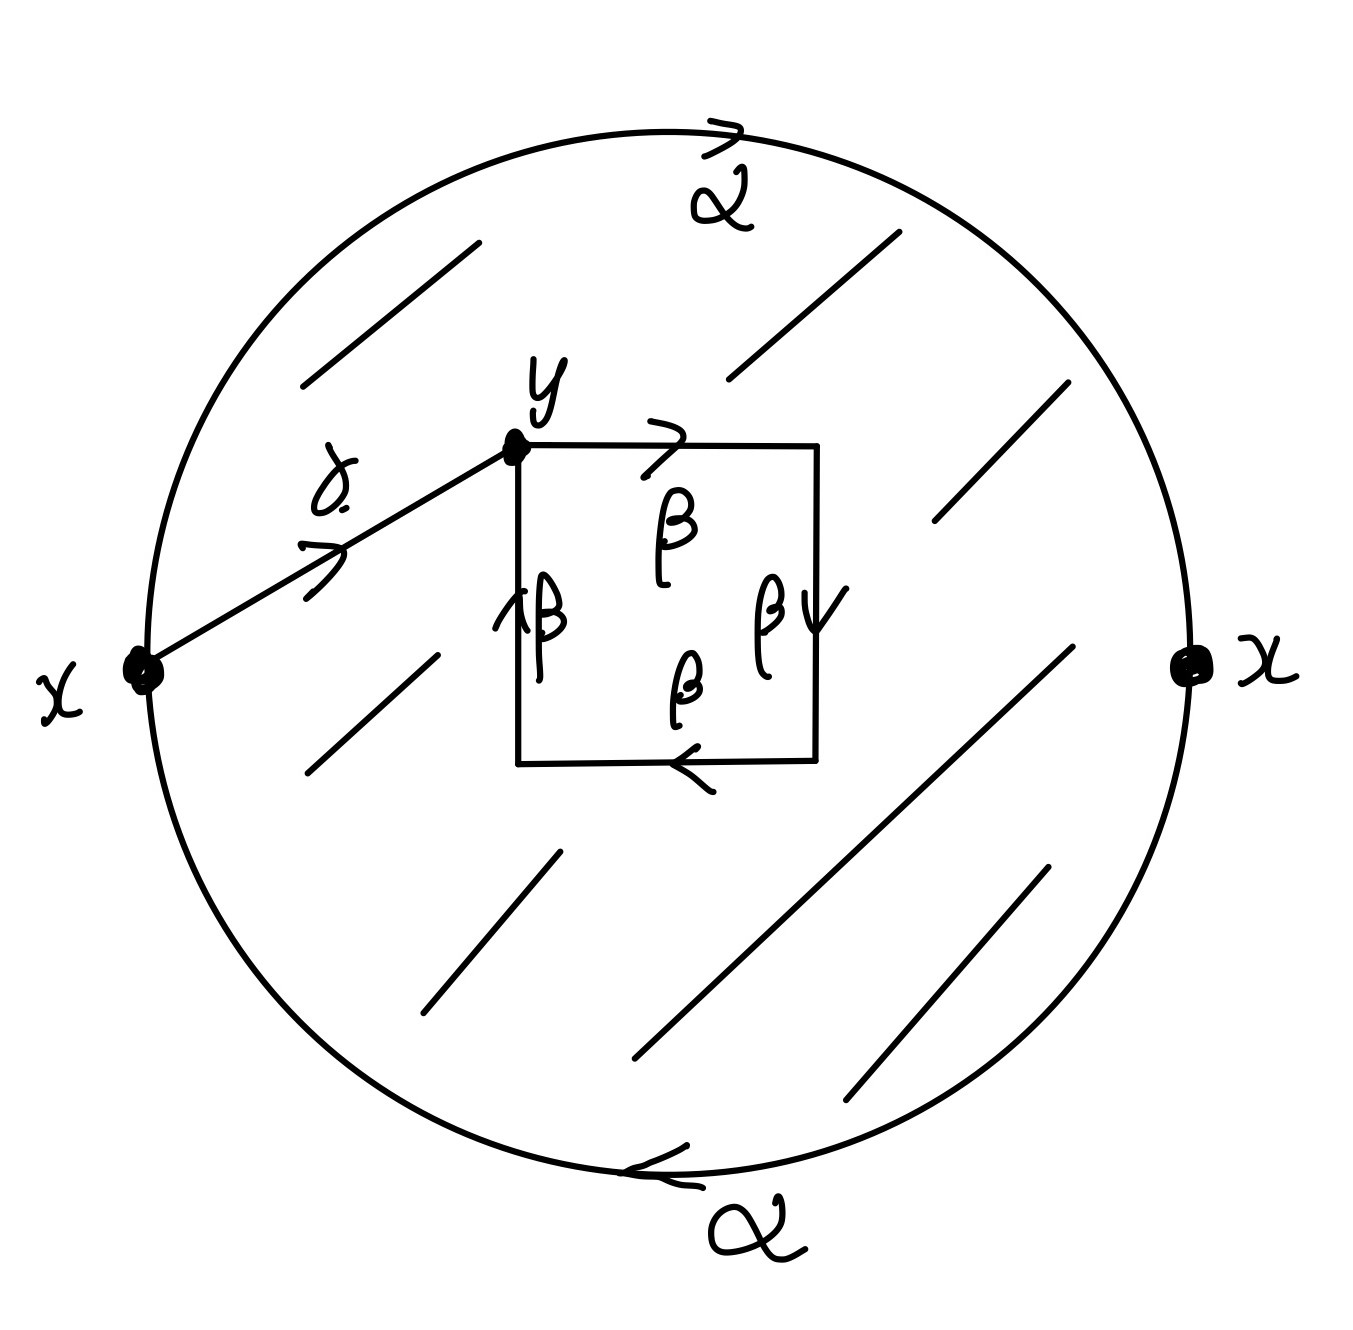
\includegraphics[scale=0.1]{Pictures/HW2-3-1.jpg}\]
We denote this space as \(Z\), which has two 0-cells \(x,y\), three 1-cells \(\alpha,\beta,\gamma\) and one 2-cell \(S\). We have the cellular chain complex:
\[\mathbb{Z}\xrightarrow{d_2}\mathbb{Z}^3\xrightarrow{d_1}\mathbb{Z}^2\xrightarrow{d_0}0.\]
The boundary maps are given by 
\begin{align*}
    d_2(S)&=2\alpha+\gamma-4\beta-\gamma=2\alpha-4\beta,\\ 
    d_1(\alpha)&=d_1(\beta)=0, d_1(\gamma)=y-x,\\ 
    d_0&=0.
\end{align*}
So we can calculate the homology group of \(Z\):
\[H_2(Z)=\ker d_2=0.\]
\begin{align*}
H_0(Z)&=\ker d_0/\im d_1\\ 
      &=\la x,y\ra/\la y-x\ra\\ 
      &=\mathbb{Z}. 
\end{align*}
and 
\begin{align*}
H_1(Z)&=\ker d_1/\im d_2\\
      &=\la \alpha,\beta\ra/\la 2\alpha-4\beta\ra\\ 
      &=\la \alpha-\beta,\alpha-2\beta\ra/\la 2(\alpha-2\beta)\ra\\ 
      &=\mathbb{Z}\oplus \mathbb{Z}/2 \mathbb{Z}.
\end{align*}
So the homology group of \(Z\) can be summarized as 
\[H_i(Z)=\begin{cases}
    \mathbb{Z},&\, \text{if}\, i=0;\\ 
    \mathbb{Z}\oplus \mathbb{Z}/2 \mathbb{Z},&\, \text{if}\, i=1;\\ 
    0,&\, \text{otherwise}.
\end{cases}\]
\end{enumerate}
\end{solution}

\noindent\rule{7in}{2.8pt}

\newpage

\begin{problem}{6}
Now that you have computed the homology of all compact \(2\)-manifolds, we can start to explore the situation for \(3\)-manifolds a bit. 
\begin{enumerate}[(a)]
\item If \(X\) is any space, recall that the suspension \(\Sigma X\) is \(CX/X\), where \(CX\) is the cone on \(X\). Prove that \(\tilde{H}_i(\Sigma X)=\tilde{H}_{i-1}(X)\) for all \(i\). 
\item If \(X\) is a pointed space then the reduced suspension \(\tilde{\Sigma}X\) is defined to be \((\Sigma X)/(\Sigma *)\) where \(*\) is the base point. Compute \(\tilde{H}_i(\tilde{\Sigma}X)\) in terms of \(\tilde{H}_i(X)\). 
\item Convince yourself there is a cofiber sequence \(S^1\vee X\hookrightarrow S^1\times X\rightarrow \tilde{\Sigma}X\). Prove that the induced maps \(H_*(S^1\vee X)\rightarrow H_*(S^1\times X)\) are injective for \(*\geq 1\) by constructing a splitting.
\item Calculate \(H_*(S^1\times T)\) and \(H_*(S^1\times \mathbb{R}P^2)\).
\end{enumerate}
\end{problem}
\begin{solution}
\begin{enumerate}[(a)]
\item The pair \((CX,X)\) is a good pair so the quotient map 
\[X\rightarrow CX\rightarrow \Sigma X\]
induces a long exact sequence in the reduced homology groups 
\[\cdots\rightarrow \tilde{H}_i(X)\rightarrow \tilde{H}_i(CX)\rightarrow \tilde{H}_i(\Sigma X)\rightarrow \tilde{H}_{i-1}(X)\rightarrow \tilde{H}_{i-1}(CX)\rightarrow \cdots\]
The space \(CX\) is contractible, so \(\tilde{H}_i(CX)=0\) for all \(i\). This implies \(\tilde{H}_i(\Sigma X)\cong \tilde{H}_{i-1}(X) \) for all \(i\). 
\item Assume for any point \(x\in X\), the pair \((X,x)\) is a good pair. Consider the inclusion \(*\hookrightarrow X\) and apply the suspension, we get the follwoing:
\[\Sigma *\hookrightarrow \Sigma X\rightarrow (\Sigma X)/(\Sigma *)\cong \tilde{\Sigma} X.\]
We have an induced long exact sequence in reduced homology groups 
\[\cdots\rightarrow \tilde{H}_i(\Sigma *)\rightarrow \tilde{H}_i(\Sigma X)\rightarrow \tilde{H}_i(\tilde{\Sigma }X)\rightarrow \tilde{H}_{i-1}(\Sigma *)\rightarrow \cdots\]
Note that \(\Sigma *\) is homeomorphic to the interval, which is contractible. So \(\tilde{H}_i(\Sigma *)=0\) for all \(i\). From the long exact sequence and (a) we can see that 
\[\tilde{H}_i(\tilde{\Sigma}X)\cong \tilde{H}_i(\Sigma X)\cong \tilde{H}_{i-1}(X)\]
for all \(i\). 
\item Identify \(S^1\times X\) as the quotient space \(Y=(I\times X)/\sim\) where \((1,x)\sim (0,x)\) for all \(x\in X\). Consider the subspace 
\[Y\supset Z=\left\{(*,t)\mid t\in I  \right\}\cup \left\{ (x,0)\mid x\in X \right\}\] 
where \(*\in X\) is the basepoint we choose. Note that \(Z\) can be viewed as \(S^1\) and \(X\) glued at the point \((*,0)\). So \(Z\cong S^1\vee X\). Moreover, 
\[\left\{ (*,t)\mid t\in I \right\}\cong \Sigma *\]
and we have 
\[\tilde{\Sigma} X=(\Sigma X)/(\Sigma *)\cong Y/Z\cong (S^1\times X)/(S^1\vee X).\]
Thus, we have a cofiber sequence \(S^1\vee X\rightarrow S^1\times X\rightarrow \tilde{\Sigma} X\).\\ 
Consider two projection maps \(p_1:S^1\times X\rightarrow S^1\) and \(p_2:S^1\times X\rightarrow X\). For all \(i\geq 1\), \(p_1\) and \(p_2\) induce maps in homology groups 
\((p_1)_*:H_i(S^1\times X)\rightarrow H_i(S^1)\) and \((p_2)_*:H_i(S^1\times X)\rightarrow H_i(X)\). Define a map 
\begin{align*}
    \phi:H_i(S^1\times X)&\rightarrow H_i(S^1)\oplus H_i(X),\\ 
         [a]&\mapsto ((p_1)_*[a],(p_2)_*[a])
\end{align*}
We can identify \(H_i(S^1\vee X)\cong H_i(S^1)\oplus H_i(X)\) and \(\phi\) can be viewed as a map \(\phi:H_i(S^1\times X)\rightarrow H_i(S^1\vee X)\). We claim this is the splitting we want. Indeed, 
write \(i:S^1\vee X\hookrightarrow S^1\times X\) as the map of inclusion and \(i_*\) is the induced map in homology, we know the composition \(\phi\circ i_*\) is induced by the following two maps of spaces:
\begin{align*}
S^1\vee X&\rightarrow S^1\times X\rightarrow S^1,\\ 
S^1\vee X&\rightarrow S^1\times X\rightarrow X.
\end{align*} 
The coproduct for two pointed spaces is the wedge sum, so we can conclude that \(\phi\circ i_*\) is indeed a splitting. And thus, \(i_*:H_i(S^1\vee X)\rightarrow H_i(S^1\times X)\) is injective for \(i\geq 1\). 
\item The cofiber sequence \(S^1\vee X\rightarrow S^1\times X\rightarrow \tilde{\Sigma}X\) induces a long exact sequence in reduced homology groups and for all \(i\geq 1\), we identify \(\tilde{H}_i(S^1\vee X)\cong \tilde{H}_i(S^1)\oplus \tilde{H}_i(X)\) 
and \(\tilde{H}_i(\tilde{\Sigma}X)\cong \tilde{H}_{i-1}(X)\) , we have 
\[\cdots\rightarrow \tilde{H}_i(S^1)\oplus \tilde{H}_i(X)\rightarrow \tilde{H}_i(S^1\times T)\rightarrow \tilde{H}_{i-1}(X)\rightarrow \tilde{H}_{i-1}(S^1)\oplus \tilde{H}_{i-1}(X)\rightarrow \cdots\]
We have shown in (c) that the map for \(i\geq 1\), \(\tilde{H}_i(S^1)\oplus \tilde{H}_i(T)\rightarrow \tilde{H}_i(S^1\times T)\) is injective, by exactness, the map 
\[\tilde{H}_{i+1}(\tilde{\Sigma}T)\cong \tilde{H}_i(T)\rightarrow \tilde{H}_i(S^1)\oplus \tilde{H}_i(T)\]
is the zero map. So for \(i\geq 2\), we have 
\[\tilde{H}_{i}(S^1\times T)/(\tilde{H}_{i}(S^1)\oplus \tilde{H}_{i}(T))\cong \tilde{H}_{i-1}(T).\]
When \(i=3\), \(\tilde{H}_3(S^1)=\tilde{H}_3(T)=0\), so 
\[H_3(S^1\times T)\cong \tilde{H}_3(S^1\times T)\cong \tilde{H}_2(T)\cong \mathbb{Z}.\]
When \(i=2\), \(\tilde{H}_2(S^1)=0\), \(\tilde{H}_2(T)=\mathbb{Z}\) and \(\tilde{H}_1(T)=\mathbb{Z}\oplus \mathbb{Z}\), so 
\[H_2(S^1\times X)\cong \mathbb{Z}\oplus \mathbb{Z}\oplus \mathbb{Z}.\]
For \(H_0(S^1\times T)\), we know that \(S^1\) and \(T\) are all path-connected, so the product \(S^1\times T\) is also path-connected. This implies that 
\[H_0(S^1\times T)\cong 0.\]
When \(i=1\), note that \(\tilde{H}_0(T)=0\), so the map 
\[i_*:\tilde{H}_1(S^1)\oplus \tilde{H}_1(T)\rightarrow \tilde{H}_0(T)\]
is an isomorphism, so 
\[H_1(S^1\times T)\cong \tilde{H}_1(S^1\times T)\cong \mathbb{Z}\oplus \mathbb{Z}\oplus \mathbb{Z}.\]
The homology group of \(S^1\times T\) can be summarized as 
\[H_i(S^1\times T)=\begin{cases}
    \mathbb{Z},&\, \text{if}\, i=0,3;\\ 
    \mathbb{Z}\oplus \mathbb{Z}\oplus \mathbb{Z},&\, \text{if}\, i=1,2;\\
    0,&\, \text{otherwise}.
\end{cases}\]

When \(X=\mathbb{R}P^2\), since \(S^1\) and \(\mathbb{R}P^2\) are path-connected, so the product \(S^1\times \mathbb{R}P^2\) are also path-connected. This implies 
\[H_0(S^1\times \mathbb{R}P^2)\cong \mathbb{Z}.\]
For \(i=2,3\), we can still use the isomorphism 
\[\tilde{H}_i(S^1\times \mathbb{R}P^2)/(\tilde{H}_i(S^1)\oplus \tilde{H}_i(\mathbb{R}P^2))\cong \tilde{H}_{i-1}(\mathbb{R}P^2).\]
Note that for \(i=2,3\), we have 
\[H_3(S^1)=H_2(S^1)=0=H_3(\mathbb{R}P^2)=H_2(\mathbb{R}P^2).\]
So 
\begin{align*}
H_3(S^1\times \mathbb{R}P^2)&\cong H_2(\mathbb{R}P^2)=0\\ 
H_2(S^1\times \mathbb{R}P^2)&\cong H_1(\mathbb{R}P^2)=\mathbb{Z}/2 \mathbb{Z}.
\end{align*}
For \(i=1\), since \(\mathbb{R}P^2\) is path-connected, so the map 
\[i_*:H_1(S^1\vee \mathbb{R}P^2)\rightarrow H_1(S^1\times \mathbb{R}P^2)\]
is an isomorphism and we have \(H_1(S^1\times \mathbb{R}P^2)=\mathbb{Z}\oplus \mathbb{Z}/2 \mathbb{Z}\). The homology groups of \(S^1\times \mathbb{R}P^2\) can be summarized as 
\[H_i(S^1\times \mathbb{R}P^2)=\begin{cases}
    \mathbb{Z},&\, \text{if}\, i=0;\\ 
    \mathbb{Z}/2 \mathbb{Z},&\, \text{if}\, i=2;\\ 
    \mathbb{Z}\oplus \mathbb{Z}/2 \mathbb{Z},&\, \text{if}\, i=1;\\ 
    0,&\, \text{otherwise}.
\end{cases}\]
\end{enumerate}
\end{solution}

\end{document}